%%%%%%%%%%%%%%%%%%%%%%%%%%%%%%%%%%%%%%%%%%%%%%%%%%%%%%%%%%%%%%%%%%%%%%%%%%%%%%%%
% Introduction
%%%%%%%%%%%%%%%%%%%%%%%%%%%%%%%%%%%%%%%%%%%%%%%%%%%%%%%%%%%%%%%%%%%%%%%%%%%%%%%%
\subsection{Introductions}
\label{anomalyDetection:commuteTime:introduction}
This section provides an overview of a method for anomaly detection using
commute time. This method was proposed by \citeauthor{Khoa:2012} in
\fullcite{Khoa:2012} \cite{Khoa:2012}. An introduction to commute time was
presented in \autoref{commuteTime}. The method described in this section forms
the base algorithm that will be implemented in hardware during this Thesis.

Commute time is an Euclidean distance in the space spanned by eigenvectors of
the graph Laplacian matrix. Commute time forms an interesting basis for an
anomaly detection algorithm because, unlike traditional Euclidean distance,
the commute time between two nodes can capture both the distance between them
and the data densities so that we can capture both global and local anomalies in
the data set \cite{Khoa:2012}.

% TODO: Replace with a tikzpicture
\begin{figure}
    \centering
    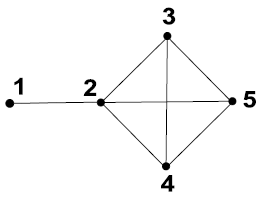
\includegraphics[width=0.3\textwidth]{commute-time/example}
    \caption{A simple example illustrating the application of commute time
        \cite{Khoa:2012}}
    \label{fig:commuteTime:example}
\end{figure}

A simple example illustrating the application of the commute time metric is
shown in \autoref{fig:commuteTime:example}. In this example, edge $e_{1,2}$ has
a larger commute time than all other edges in the cluster, whilst its Euclidean
distance is the same or smaller than the neighbouring Euclidean distances.

A key property of the commute time metric that allows for its use for anomaly
detection is that, by adding more data points to an existing cluster (i.e.,
making the cluster more dense), the commute time between anomalous data points
and the cluster changes dramatically whilst the average pair-wise commute times
of all nodes within the cluster is largely unaffected. This property is
illustrated in \autoref{fig:commuteTime:example2}.

% TODO: Replace with a tikzpicture
\begin{figure}
    \centering
    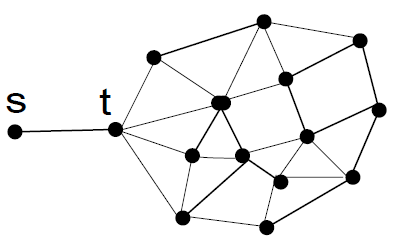
\includegraphics[width=0.3\textwidth]{commute-time/example2}
    \caption{The commute distance from an anomaly ($s$) to a node in a cluster
        ($t$) increases when the cluster is denser \cite{Khoa:2012}}
    \label{fig:commuteTime:example2}
\end{figure}

\citeauthor{Khoa:2012} was able to devise and prove an anomaly detection
algorithm (using the commute time metric) to detect global and local outliers.
Extending this algorithm, \citeauthor{Khoa:2012} was able to use graph component
sampling and Eigenspace approximation in order to avoid the $O(n^3)$ Eigen
decomposition of the graph Laplacian. Furthermore, a pruning technique was used
in attempt to improve the run time complexity of the algorithm to $O(n\log n)$.

%%%%%%%%%%%%%%%%%%%%%%%%%%%%%%%%%%%%%%%%%%%%%%%%%%%%%%%%%%%%%%%%%%%%%%%%%%%%%%%%
% Anomaly Detection Using Commute Time
%%%%%%%%%%%%%%%%%%%%%%%%%%%%%%%%%%%%%%%%%%%%%%%%%%%%%%%%%%%%%%%%%%%%%%%%%%%%%%%%
\subsection{Anomaly Detection Using Commute Time}
\label{anomalyDetection:commuteTime:algorithm}
The algorithm proposed by \citeauthor{Khoa:2012} in \fullcite{Khoa:2012}
\cite{Khoa:2012} is presented in \autoref{algm:anomalyDetection:commuteTime}.
This section describes in detail each stage of the algorithm.

\begin{algorithm}[t]
    % TODO
\LinesNumbered

\SetKwInput{InputK}{k}
\SetKwInput{InputN}{N}
\SetKwInput{InputD}{Data}
\SetKwInOut{OutputO}{outliers}

\InputK{the number of nearest neighbors}
\InputN{the number of outliers to return}
\InputD{a set of examples in random order}
\OutputO{a set of outliers}

\SetKwData{varB}{b}
\SetKwData{Block}{block}
\SetKwData{Cutoff}{cutoff}
\SetKwData{varD}{d}
\SetKwData{Data}{Data}
\SetKwData{varK}{k}
\SetKwData{varN}{N}
\SetKwData{Neighbours}{neighbours}
\SetKwData{varO}{o}
\SetKwData{Outliers}{outliers}
\SetKwData{Score}{score}

\SetKwFunction{Closest}{closest}
\SetKwFunction{Distance}{distance}
\SetKwFunction{GetNextBlock}{getNextBlock}
\SetKwFunction{MaxDist}{maxDist}
\SetKwFunction{Min}{min}
\SetKwFunction{Top}{top}

\Begin{
    $\Cutoff \longleftarrow 0$\tcp*[l]{set the cutoff for pruning to $0$}
    $\Outliers \longleftarrow \emptyset$\tcp*[l]{initialize to the empty set}
    \BlankLine
    \While(\tcp*[h]{load a block of examples from \varD}){$\Block \longleftarrow \GetNextBlock{\Data}$}{
        $\Neighbours(\varB) \longleftarrow \emptyset, \quad \forall \, \varB \in \Block$\;
        \BlankLine
        \ForEach{$\varD \in \Data$}{
            \ForEach{$\varB \in \Block \: : \: \varB \neq \varD$}{
                \If{$|\Neighbours(\varB)| < \varK \: \lor \: \Distance{\varB, \varD} < \MaxDist{\varB, \Neighbours(\varB)}$}{
                    $\Neighbours(\varB) \longleftarrow \Closest{\varB, \Neighbours(\varB)} \cup \varD, \varK)$\;
                    \If{$\Score(\Neighbours(\varB), \varB) < \Cutoff$}{
                        $\Block \longleftarrow \Block \setminus \varB$\;
                    }
                }
            }
        }
        \BlankLine
        $\Outliers \longleftarrow $\Top{$\Block \cup \Outliers$, $\varN$}\tcp*[l]{keep only the top n outliers}
        $\Cutoff \longleftarrow \Min_{\varO \in \Outliers}(\Score(\varO))$\tcp*[l]{the cutoff is the score of the weakest outlier}
    }
    \KwRet{\Outliers}\;
}

    \caption{Anomaly Detection using Commute Time}
    \label{algm:anomalyDetection:commuteTime}
\end{algorithm}

% Construction of the k-Nearest Neighbour Graph
\subsubsection{Construction of the $k$-Nearest Neighbour Graph}
\label{anomalyDetection:commuteTime:algorithm:knnGraph}
The first stage of the algorithm is to compute the $k$-nearest neighbour graph
for the input data set.

For this purpose, the $kd$-tree technique can be applied so as to avoid an
$O(n^2)$ searching of nearest neighbours.